% ---- BEGIN monograph/chapters/04_tensor_scalar_temporal_field.tex ----
\chapter{Tensor--Scalar Temporal Field}
The temporal configuration is represented by a scalar pace together with a rank-two relational response sector. The scalar component is typed by the internal elapsed density
\[
\boxed{
\phi
=\frac{d\tau_{\rm int}}{d\lambda}
=\frac{\mathfrak a}{\mathfrak a_\star}>0.
}
\]
For the same ordering increment \(d\lambda\), distinct admitted relational states may therefore realize distinct internal elapsed increments.

The tensorial response is written locally as
\[
\boxed{
\mathcal R^{AB}=G^{AB}+\Omega^{AB},
}
\]
where
\[
G^{AB}=G^{BA},
\qquad
\Omega^{AB}=-\Omega^{BA}.
\]
The symmetric positive sector maps the informational covector to dissipative state transport,
\[
V_I^A=-G^{AB}\partial_B\mathcal I,
\]
while the antisymmetric sector maps a local exact phase covector to reversible state transport,
\[
V_H^A=\Omega^{AB}\partial_B\mathcal H_\alpha.
\]

Formalism 01C supplies the stationary Shannon informational scalar
\[
\boxed{
\mathcal I_\pi[p]=D_{\rm KL}^{(2)}(p\|\pi).
}
\]
For admitted stationary transition dynamics this scalar contracts. In the detailed-balance sector, Formalism 01D derives the exact symmetric response
\[
\boxed{
G^{(2)}_\pi(p)
=(\ln2)D^\top\operatorname{diag}[c_{ab}\Lambda(r_a,r_b)]D,
\qquad
r_a=\frac{p_a}{\pi_a},
}
\]
and the exact flow identity
\[
\boxed{
\dot p=-G^{(2)}_\pi(p)\nabla_p\mathcal I_\pi.
}
\]
The mass-conservation direction satisfies
\[
G^{(2)}_\pi\mathbf1=0,
\]
so the corresponding metric response is taken on the active simplex tangent quotient. At uniform zero-drive equilibrium,
\[
\boxed{
G^{(2)}_u(u)=\frac{\ln2}{m}K_0,
}
\]
which ties the symmetric information-response tensor directly to the relational-mobility Laplacian used by Temporal Wave.

In the admitted Kähler factorization on a compatible active sector,
\[
g_{K,AB}=(G^{-1})_{AB},
\qquad
\Omega^{AB}=J^A{}_{C}G^{CB},
\]
where the inverse is understood on the nondegenerate tangent sector when conservation constraints are present. On an exact phase patch the evolution law is
\[
\boxed{
\frac{dx}{d\lambda}
=-\operatorname{grad}_{g_K}\mathcal I
+J\operatorname{grad}_{g_K}\mathcal H_\alpha.
}
\]
This form is the coordinate-covariant factorization of the symmetric informational-response channel and the antisymmetric local phase-response channel established in Formalism 01A.

Formalism 01B supplies the global phase completion. The edge link
\[
L_e=G_e\exp\!\left[i\kappa(\Delta H_e+\sigma_e)\right]
\]
defines a temporal connection class whose closed-cycle holonomy is
\[
\boxed{
\Phi_T(C)=\gamma_B(C)+\kappa\sum_{e\in C}\sigma_e\pmod{2\pi}.
}
\]
The exact Shannon part telescopes on a closed cycle. Berry holonomy and non-exact affinity provide the global connection data. Thus \(\mathcal H_\alpha\) is typed as a local exact-patch generator, while the U(1) connection carries global phase patching and cycle information.

The tensor--scalar temporal architecture is therefore summarized locally by
\[
\boxed{
\mathcal T
=\bigl(\phi,\mathcal R^{AB}\bigr),
\qquad
\phi=\frac{\mathfrak a}{\mathfrak a_\star},
\qquad
\mathcal R^{AB}=G^{AB}+J^A{}_{C}G^{CB},
}
\]
with a global phase-connection layer supplying the holonomy class. The scalar answers how much internal elapsed time is realized per ordering increment. The symmetric tensorial sector has a Shannon--Onsager realization in probability coordinates, while the antisymmetric/connection sector carries orientation and circulation.

The next upstream task is to extend the response decomposition to stationary nonreversible dynamics while retaining the 01C relative-information contraction and the 01B connection/current structure. Downstream realizations are tested through Temporal Wave, NOW, Bifurcation, Transport, Memory and Retrodiction.

\section{nD slices of the tensor--scalar field}
Because the full tensor--scalar state lives in a space of dimension higher than two, Figure~\ref{fig:nd-slices} provides four schematic two-dimensional slices as a readable proxy for the richer field geometry.
\begin{figure}[H]
  \centering
  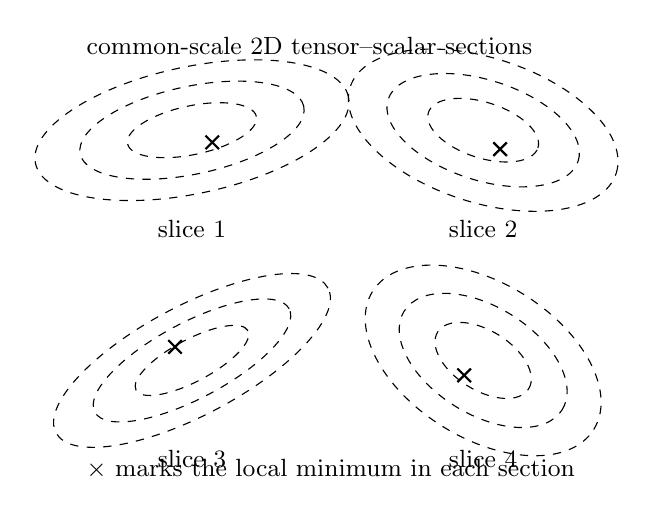
\begin{tikzpicture}[scale=0.86]
    \foreach \x/\y/\ang/\sx/\sy/\mx/\my/\lab in {
      -3.3/2.0/12/1.35/0.72/-3.0/1.82/{slice 1},
       1.0/2.0/-18/1.18/0.82/1.25/1.72/{slice 2},
      -3.3/-1.4/28/1.30/0.62/-3.55/-1.20/{slice 3},
       1.0/-1.4/-32/1.10/0.88/0.72/-1.62/{slice 4}}
    {
      \begin{scope}[shift={(\x,\y)},rotate=\ang]
        \draw[dashed] (0,0) ellipse ({1.75*\sx} and {1.30*\sy});
        \draw[dashed] (0,0) ellipse ({1.25*\sx} and {0.90*\sy});
        \draw[dashed] (0,0) ellipse ({0.72*\sx} and {0.50*\sy});
      \end{scope}
      \draw[thick] (\mx-0.10,\my-0.10) -- (\mx+0.10,\my+0.10);
      \draw[thick] (\mx-0.10,\my+0.10) -- (\mx+0.10,\my-0.10);
      \node[font=\small] at (\x,\y-1.45) {\lab};
    }
    \node[font=\small,anchor=west] at (-5.0,3.25) {common-scale 2D tensor--scalar sections};
    \node[font=\small,anchor=west] at (-5.0,-3.0) {$\times$ marks the local minimum in each section};
  \end{tikzpicture}
  \caption{Schematic four common-scale two-dimensional slices of a higher-dimensional tensor--scalar surrogate. The fixed tensor coordinates deform the local informational landscape; the cross marks the minimum in each slice.}
  \label{fig:nd-slices}
\end{figure}

% ---- END monograph/chapters/04_tensor_scalar_temporal_field.tex ----

% ---- BEGIN monograph/chapters/05_chiral_fractal_temporal_topology.tex ----
\chapter[Chiral--Fractal Temporal Topology]{Chiral--Fractal Temporal Topology as a Derived-Property Gate}
The Neutrinotime line motivates a fractal--chiral temporal topology as a comparison target. In the present derivation, the target is decomposed into independently testable quantities:
\[
I_{\rm top}[\Gamma],\qquad \chi[\Gamma],\qquad D_F[\Gamma].
\]
These denote, respectively, a topological invariant, a signed chirality/orientation observable, and a fractal-scaling observable of an orbit or invariant set \(\Gamma\).

A minimal chirality candidate is a signed holonomy,
\[
\chi[C]=\operatorname{sgn}\!\left(\oint_C A\right),
\]
whenever the dynamical state bundle supplies an admitted connection \(A\). Orientation reversal must reverse the sign of \(\chi\) while declared non-chiral invariants remain unchanged.

Fractality is measured prospectively from the derived tensor--scalar dynamics through \(D_F\), a renormalization relation, a Lyapunov diagnostic, or another explicit scaling test. A linear Kähler control supplies the non-fractal reference class.

The relation between event-localized NOW and a dynamical bifurcation locus remains an open bridge. They are maintained as separate typed objects until an equivalence theorem or prospective experiment closes that dependency.

\section{Visual intuition for chirality and event structure}
The schematic rendering in Figure~\ref{fig:temporal-ribbon-3d} shows a single trajectory lifted over an informational landscape, making visible the joint role of orbital phase and informational descent. Figure~\ref{fig:event-measure} then shows a schematic discrete event measure extracted from an evolving informational signal.
\begin{figure}[H]
  \centering
  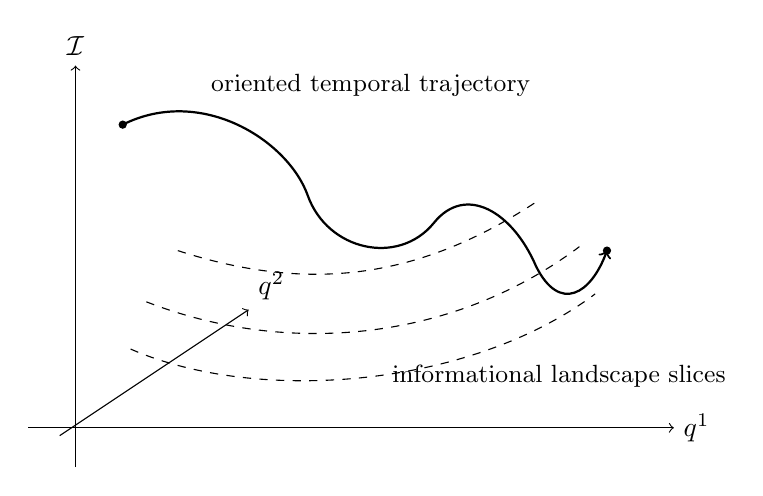
\begin{tikzpicture}[scale=1.0]
    \draw[->] (-4.0,-1.9) -- (4.2,-1.9) node[right] {$q^1$};
    \draw[->] (-3.4,-2.4) -- (-3.4,2.7) node[above] {$\mathcal I$};
    \draw[->] (-3.6,-2.0) -- (-1.2,-0.4) node[above right] {$q^2$};
    \draw[dashed] (-2.7,-0.9) .. controls (-1.1,-1.6) and (1.6,-1.4) .. (3.2,-0.2);
    \draw[dashed] (-2.5,-0.3) .. controls (-0.7,-1.0) and (1.4,-0.8) .. (3.0,0.4);
    \draw[dashed] (-2.1,0.35) .. controls (-0.4,-0.2) and (1.0,0.0) .. (2.5,1.0);
    \draw[->,thick]
      (-2.8,1.95)
      .. controls (-1.8,2.45) and (-0.7,1.75) .. (-0.45,1.05)
      .. controls (-0.20,0.35) and (0.70,0.15) .. (1.15,0.70)
      .. controls (1.55,1.20) and (2.15,0.85) .. (2.45,0.15)
      .. controls (2.75,-0.45) and (3.15,-0.20) .. (3.35,0.35);
    \fill (-2.8,1.95) circle (1.5pt);
    \fill (3.35,0.35) circle (1.5pt);
    \node[font=\small,anchor=west] at (-1.8,2.45) {oriented temporal trajectory};
    \node[font=\small,anchor=west] at (0.5,-1.25) {informational landscape slices};
  \end{tikzpicture}
  \caption{Schematic lifted slice of temporal evolution on the Kähler informational landscape. The vertical coordinate represents the informational functional $\mathcal{I}$ along an oriented trajectory.}
  \label{fig:temporal-ribbon-3d}
\end{figure}
\begin{figure}[H]
  \centering
  \begin{tikzpicture}[x=0.92cm,y=1.0cm]
    \draw[->] (0,0) -- (11.2,0) node[right] {$\lambda$};
    \draw[->] (0,-0.2) -- (0,3.0) node[above] {event weight};
    \draw[dashed] (0,1.0) -- (10.7,1.0) node[right,font=\small] {reference level};
    \foreach \x/\h in {0.7/0.35,1.5/0.75,2.4/0.45,3.2/1.55,4.0/0.65,5.1/2.35,6.0/0.55,6.9/1.25,7.8/0.50,8.9/1.90,9.8/0.70}
      \draw[thick] (\x,0) -- (\x,\h);
    \foreach \x/\h in {3.2/1.55,5.1/2.35,6.9/1.25,8.9/1.90}
      \fill (\x,\h) circle (1.8pt);
    \node[font=\small,anchor=west] at (3.35,2.65) {localized event support};
  \end{tikzpicture}
  \caption{Schematic discrete event measure on the ordering parameter. Selected localized peaks illustrate the event-support coordinate used to compare temporal evolution with NOW localization.}
  \label{fig:event-measure}
\end{figure}

% ---- END monograph/chapters/05_chiral_fractal_temporal_topology.tex ----

% ---- BEGIN monograph/chapters/03_nature_of_temporal_state.tex ----
\chapter{Nature of the Temporal State}

The temporal architecture developed here begins with directed relational composability rather than an assumed temporal order. Realized relations form composable words. Their prefixes define distinct history occurrences, positive transition activity supplies an intrinsic duration weight, and the combination produces temporal precedence. NOW is then the maximal supported frontier of the realized occurrence history. A downstream half-frame construction provides a finite-support realization in which neighboring temporal frames overlap while preserving the total intrinsic elapsed measure.

\section{Pretime relational composition}

Let
\[
\mathcal G=(S,E,s,t)
\]
be a directed relational multigraph. An edge $e:a\to b$ carries source and target labels. Two relations compose when
\[
\boxed{t(e_k)=s(e_{k+1}).}
\]
A finite realized word is
\[
\boxed{
P_n=e_n\circ\cdots\circ e_1,
}
\]
with prefixes
\[
P_0=\mathrm{id},
\qquad
P_k=e_k\circ\cdots\circ e_1.
\]
Define the realized occurrence
\[
\boxed{\nu_k=(P_k,x_k),}
\]
where $x_k$ is the terminal state label of $P_k$. Repeated state labels remain distinct occurrences because the full prefixes differ.

Define the prefix relation
\[
\boxed{
\nu_i\sqsubseteq\nu_j
\iff
\exists Q:\ P_j=Q\circ P_i.
}
\]
On prefix-labelled occurrences it is reflexive, transitive and antisymmetric. Along one realized serial word it is total.

\section{Transition traffic and intrinsic duration}

For an admitted active pair,
\[
W_+=Me^{A/2},
\qquad
W_-=Me^{-A/2},
\qquad M>0,
\]
and therefore
\[
\boxed{\mathfrak a=W_++W_-=2M\cosh(A/2)>0,}
\]
\[
\boxed{\mathfrak j=W_+-W_-=2M\sinh(A/2).}
\]
Independent-channel extensivity, continuity and invariance of duration under orientation exchange force the local duration density to have the form
\[
F(W_+,W_-)=C(W_++W_-),
\qquad C>0.
\]
In intrinsic activity units $C=1$.

For any increasing local edge parameter $\lambda_e$,
\[
\boxed{
\theta(e)=\int_e\mathfrak a\,d\lambda_e>0
}
\]
is invariant under admitted reparameterization. The infinitesimal form is
\[
\boxed{d\Theta=\mathfrak a\,d\lambda_e.}
\]
For a realized prefix,
\[
\boxed{
\Theta(P_k)=\sum_{r=1}^{k}\theta(e_r).
}
\]
Hence a strict prefix extension obeys
\[
\boxed{
\nu_i\sqsubset\nu_j
\Longrightarrow
\Theta(P_i)<\Theta(P_j).
}
\]
On one serial word the converse holds. Temporal precedence is therefore defined on realized occurrences by
\[
\boxed{
\nu_i\prec_T\nu_j
\iff
\nu_i\sqsubset\nu_j,
}
\]
with $\Theta$ providing its strictly increasing scalar realization.

\section{Recurrence and temporal advance}

A relational cycle in state labels,
\[
A\to B\to A,
\]
produces
\[
(A,P_0)\prec_T(B,P_1)\prec_T(A,P_2).
\]
Thus the state label can recur while the realized occurrence history continues to advance. The distinction between state identity and occurrence identity is retained by the full relation prefix.

\section{Duration and orientation}

The normalized directional coordinate is
\[
\boxed{
\chi=\frac{\mathfrak j}{\mathfrak a}=\tanh(A/2).
}
\]
Using the Shannon affinity in bits,
\[
A=(\ln2)\sigma,
\]
we obtain
\[
\boxed{
\chi=\tanh\!\left(\frac{\ln2}{2}\sigma\right)
}
\]
and
\[
\boxed{
d\Theta=2M\cosh\!\left(\frac{\ln2}{2}\sigma\right)d\lambda_e.}
\]
Under orientation reversal $A\mapsto-A$, duration is even and $\chi$ is odd. At $A=0$,
\[
\boxed{\theta(e)>0,\qquad \chi=0.}
\]
The accumulated duration coordinate and the local directional-affinity coordinate are therefore distinct.

With
\[
M_{ab}
=\frac{\sqrt{\rho_R(a)\rho_R(b)}}{\tfrac12[\eta_R(a)+\eta_R(b)]},
\]
the intrinsic duration density becomes
\[
\boxed{
\frac{d\Theta}{d\lambda_e}
=
2\frac{\sqrt{\rho_R(a)\rho_R(b)}}{\tfrac12[\eta_R(a)+\eta_R(b)]}
\cosh\!\left(\frac{\ln2}{2}\sigma_{ab}\right).
}
\]

\section{Half-frame temporal gluing}

Let a finite serial sector contain $N$ discrete temporal frames. Associate the phase budget
\[
\boxed{\Phi_N=2\pi N.}
\]
Each frame is split into two half-supports,
\[
\boxed{
|n\rangle
\mapsto
\frac{|n,L\rangle+|n,R\rangle}{\sqrt2}.
}
\]
Neighboring halves are identified by
\[
\boxed{|n,R\rangle\sim|n+1,L\rangle.}
\]
The resulting support sequence has $N+1$ elements,
\[
\boxed{
|1|,\ |12|,\ |23|,\ldots,\ |N-1,N|,\ |N|.
}
\]
The first modular sectors therefore read
\[
\begin{aligned}
2\pi &: \quad |1|1|,\\
4\pi &: \quad |1|12|2|,\\
6\pi &: \quad |1|12|23|3|,\\
8\pi &: \quad |1|12|23|34|4|.
\end{aligned}
\]
The counting identity is
\[
\boxed{2N-(N-1)=N+1.}
\]

For frame amplitudes $a_n$, the neighboring overlap and antisymmetric seam amplitudes are
\[
\boxed{
b_n=\frac{a_n+a_{n+1}}2,
\qquad
d_n=\frac{a_n-a_{n+1}}2.
}
\]
Together with the two boundary amplitudes they satisfy the exact norm decomposition
\[
\boxed{
\sum_{j=0}^{N}|b_j|^2
+\sum_{n=1}^{N-1}|d_n|^2
=\sum_{n=1}^{N}|a_n|^2.
}
\]
Equal neighboring phase therefore occupies the overlap support, while opposite neighboring phase produces an interface null and transfers weight into the seam-defect sector.

The same topology acts on the positive activity-derived elapsed measure. For frame intervals $\theta_n>0$, define
\[
\boxed{\ell_0=\frac{\theta_1}{2},}
\]
\[
\boxed{\ell_n=\frac{\theta_n+\theta_{n+1}}2,
\qquad 1\le n<N,}
\]
and
\[
\boxed{\ell_N=\frac{\theta_N}{2}.}
\]
Then
\[
\boxed{
\sum_{j=0}^{N}\ell_j
=\sum_{n=1}^{N}\theta_n
=\Theta_N.
}
\]
Thus neighboring overlap redistributes temporal support while preserving the total intrinsic elapsed measure exactly.

\section{Half-frame path complex and long-wave topology}

The $N+1$ glued supports form vertices $v_0,\ldots,v_N$. Each full temporal frame becomes one oriented edge
\[
\boxed{e_n=[v_{n-1},v_n].}
\]
Hence the half-frame quotient generates the path complex $P_{N+1}$. Its incidence operator is
\[
\boxed{\partial_1 e_n=v_n-v_{n-1}.}
\]
For positive frame weights $w_n$, the support Laplacian is
\[
\boxed{
L_V=D_N\operatorname{diag}(w_n)D_N^T,
}
\]
with
\[
L_V=L_V^T,
\qquad
L_V\succeq0,
\qquad
L_V\mathbf1=0.
\]
For uniform $w_n=w$, its exact spectrum is
\[
\boxed{
\lambda_k
=2w\left[1-\cos\left(\frac{k\pi}{N+1}\right)\right],
\qquad k=0,\ldots,N.
}
\]
The low sector approaches
\[
\boxed{
\lambda_k
=w\left(\frac{k\pi}{N+1}\right)^2
+O\!\left(\frac{k^4}{(N+1)^4}\right).
}
\]
This provides the topological origin of the local path incidence used by the discrete Temporal Wave coarse-graining sector.

\section{NOW as the maximal realized frontier}

For an admitted transition edge define the gauge-invariant event signature
\[
\boxed{
q_e=
\sqrt{
 d_{FS}(a,b)^2+
 \kappa^2\Delta H_e^2+
 \kappa^2\sigma_e^2
 }\ge0.
}
\]
The nonzero event carrier is
\[
\mathcal E_q
=\operatorname{supp}_{\rm at}
\left(\sum_e q_e\delta_{s_e}\right).
\]
For a finite realized down-set $D$ of occurrence prefixes, define
\[
D_q=\{\nu\in D:q_{e(\nu)}>0\}.
\]
Then
\[
\boxed{
\mathcal N(D)
=\operatorname{Max}_{\prec_T}(D_q).
}
\]
For a serial history the frontier contains the latest supported occurrence. For independent concurrent branches it is the antichain of maximal supported occurrences.

The half-frame path gives a concrete serial realization of the same rule. At stage $N$ the terminal pure support is
\[
\boxed{\mathrm{NOW}_N\leftrightarrow|N|_\partial.}
\]
When frame $N+1$ is realized,
\[
\boxed{
|N|_\partial
\longmapsto
|N,N+1|,
\qquad
\mathrm{NOW}_{N+1}\leftrightarrow|N+1|_\partial.
}
\]
The previous boundary is thereby incorporated into the neighboring-history interface while the newly created right boundary becomes the maximal serial support.

At the level of elapsed measure, if the new frame carries $\theta_{N+1}>0$, the support extension increases the total measure by exactly
\[
\boxed{\Delta\Theta=\theta_{N+1}.}
\]
Thus the half-frame moving frontier and the prefix-extension ordering share the same positive one-step temporal increment.

\section{Relative clocks and calibrated elapsed time}

For two active subsystems on a common relational comparison patch,
\[
\boxed{
N_R(x|r)
=\frac{d\Theta_x}{d\Theta_r}
=\frac{\mathfrak a_x}{\mathfrak a_r}>0.
}
\]
Reference changes compose multiplicatively,
\[
N_{x|s}=N_{x|r}N_{r|s}.
\]
A physical reference-clock calibration supplies the conversion scale,
\[
\boxed{dt=T_r\,d\Theta_r,}
\]
and therefore
\[
\boxed{d\hat\tau_x=N_Rdt.}
\]
On the admitted lapse/phase-rate bridge,
\[
\boxed{r_t=N_Rr_n^{(\tau)}.}
\]

\section{Phase topology, bifurcation and transport}

The information--phase link is
\[
L_e
=G_e\exp\!\left[i\kappa(\Delta H_e+\sigma_e)\right],
\qquad
\boxed{\kappa=\frac{\ln2}{24\pi}}.
\]
On a closed cycle,
\[
\boxed{
\operatorname{Arg}\prod_{e\in C}L_e
=\gamma_B(C)+\kappa\sum_{e\in C}\sigma_e
\pmod{2\pi}.
}
\]
At a supported maximal event occurrence the state update is represented by
\[
\boxed{
\Psi_T(s_n^+)=B_n\Psi_T(s_n^-).
}
\]
Between event occurrences,
\[
\boxed{\Psi_{n+1}=U_n\Psi_n.}
\]
A realized operator word has the compositional form
\[
\boxed{
\Psi_N
=U_{N-1}B_{N-1}\cdots U_2B_2U_1B_1\Psi_0.
}
\]
The operator composition and the relational occurrence prefix carry the same realized lineage order.

Within the Zeta--Collatz Temporal Wave candidate, a Hermitian frame Hamiltonian acts on the already-derived intrinsic coordinate,
\[
\boxed{
i\partial_\Theta a(\Theta)=H_{\zeta C}a(\Theta).
}
\]
The half-frame quotient then supplies the topology-driven interface readout. In the declared five-frame reference witness, a sharp initial frame has raw neighboring-interface occupancy $F_{1/2}(0)=0.25$, while the evolved state at the declared intrinsic interval reaches an occupancy above $0.5$. This is retained as a finite reference witness of dynamical frame-to-interface spreading; general dynamical classification remains subject to its separate gate.

\section{Memory and retrodiction}

Memory retains the realized occurrence lineage together with its temporal carriers. ORCHORBITAL records the active-attractor sequence
\[
\alpha=(a_1,\ldots,a_N),
\]
signed winding
\[
\mathcal W=(\Delta W_1,\ldots,\Delta W_N),
\]
and residence-bound radial lineage
\[
\mathcal R=(\rho_1,\ldots,\rho_N).
\]
Retrodiction reconstructs hidden histories on these retained strata. Spatial Offset Divergence audits collision fibres of compressed observation maps, while the cumulative coordinate $\Theta(P_k)$ supplies the intrinsic duration carried by the same realized prefix history.

\section{Derived temporal architecture}

The present derivation is
\[
\boxed{
\begin{aligned}
&\text{DIRECTED RELATIONAL COMPOSABILITY}\\
&\downarrow\\
&\text{REALIZED WORDS AND PREFIX OCCURRENCES}\\
&\downarrow\\
&\mathfrak a=W_++W_-,\quad \mathfrak j=W_+-W_-\\
&\downarrow\\
&\theta(e)=\int_e\mathfrak a\,d\lambda_e,\quad
\Theta(P)=\sum_e\theta(e),\quad
\chi=\mathfrak j/\mathfrak a\\
&\downarrow\\
&\text{TEMPORAL PRECEDENCE FROM PREFIX EXTENSION}\\
&\downarrow\\
&\text{TEMPORAL WAVE / HALF-FRAME OVERLAP SUPPORT}\\
&\downarrow\\
&\text{NOW}=\operatorname{Max}(\text{SUPPORTED REALIZED OCCURRENCES})\\
&\downarrow\\
&\text{BIFURCATION}\to\text{TRANSPORT}\to\text{MEMORY}\to\text{RETRODICTION}.
\end{aligned}
}
\]
Physical clock calibration, spin-$1/2$/four-$\pi$ binding and downstream spacetime closure retain their declared evidence gates.

% ---- END monograph/chapters/03_nature_of_temporal_state.tex ----

% ---- BEGIN monograph/chapters/04_wave_structure_of_time.tex ----
\chapter{Wave Structure of Time}

The relational transition layer carries a unit-modulus phase link $L_{ab}\in U(1)$ and a positive symmetric mobility $M_{ab}$.  For an oriented edge $e:a\to b$, define the covariant difference
\[
(D_L\Phi)_{ab}=\Phi_b-L_{ab}\Phi_a.
\]
The associated positive quadratic form is
\[
\mathcal E_W[\Phi]
=\sum_e M_e |(D_L\Phi)_e|^2,
\]
which defines the Hermitian positive-semidefinite Temporal Wave operator
\[
\boxed{
K_M=D_L^\dagger\operatorname{diag}(M_e)D_L.
}
\]
The mobility is inherited from the relational kinetic pair,
\[
M_{ab}
=\frac{\sqrt{\rho_R(a)\rho_R(b)}}{\tfrac12[\eta_R(a)+\eta_R(b)]}.
\]
Thus the wave stiffness uses the same positive coefficient that controls the symmetric transition rate at zero antisymmetric drive.

\section{Relational viscosity and damping}

Let
\[
\bar\eta_{ab}=\frac{\eta_R(a)+\eta_R(b)}2.
\]
The viscosity-weighted covariant operator is
\[
\boxed{
C_\eta
=D_L^\dagger\operatorname{diag}(\bar\eta_e)D_L.
}
\]
For conjugate wave coordinates $(q,p)$, the tested candidate evolution is
\[
\dot q=-p,
\qquad
\dot p=K_Mq-C_\eta p,
\]
or equivalently
\[
\boxed{
\ddot q+C_\eta\dot q+K_Mq=0.
}
\]
With
\[
\mathcal H_T
=\frac12p^\dagger p+\frac12q^\dagger K_Mq,
\]
the exact balance is
\[
\boxed{
\frac{d\mathcal H_T}{d\lambda}
=-p^\dagger C_\eta p\le0.
}
\]

\section{Heterogeneous long-wave limit}

For a one-dimensional periodic heterogeneous relational cell, let $M_e$ and $\eta_e$ denote the edge mobility and pair viscosity.  The acoustic cell corrector yields
\[
\boxed{
M_{\rm eff}
=\left\langle M_e^{-1}\right\rangle^{-1}
}
\]
and
\[
\boxed{
\beta_{\rm eff}
=M_{\rm eff}^2
\left\langle\frac{\eta_e}{M_e^2}\right\rangle.
}
\]
The long-wave positive-frequency branch is therefore
\[
\boxed{
\omega(k)
=\sqrt{M_{\rm eff}}\,|k|
-i\frac{\beta_{\rm eff}}2k^2
+O(|k|^3).
}
\]
For uniform relational fields,
\[
M_{\rm eff}=\frac{\rho_0}{\eta_0},
\qquad
\beta_{\rm eff}=\eta_0.
\]

\section{Holonomy shift}

For total closed-cell phase $\phi$ and Bloch phase $\theta$, the tested heterogeneous branch depends on the shifted wave number
\[
\boxed{
k_{\rm eff}=\frac{\operatorname{wrap}(\theta-\phi)}{L}.
}
\]
Hence
\[
\boxed{
\omega
=\sqrt{M_{\rm eff}}\,|k_{\rm eff}|
-i\frac{\beta_{\rm eff}}2k_{\rm eff}^2+\cdots.
}
\]
On a uniform $N$-cycle the exact spectrum is
\[
\lambda_m
=4MN^2
\sin^2\!\left(\frac{2\pi m-\phi}{2N}\right),
\]
so a nontrivial principal holonomy opens a positive lowest-mode gap.

These results provide the upstream wave carrier consumed by the NOW localization layer.  Metric-clock calibration remains assigned to the later Einstein-closure stage of the dependency graph.

% ---- END monograph/chapters/04_wave_structure_of_time.tex ----

% ---- BEGIN monograph/chapters/05_now.tex ----
\chapter{NOW as a Positive Wave-Active Transition Support}

The NOW layer separates structural event signature, kinetic pace, directional current and dynamical wave activation.

\section{Structural transition signature}

For an admitted transition edge $e:a\to b$, define
\[
\boxed{
q_e=
\sqrt{
 d_{FS}(a,b)^2
 +\kappa^2\Delta H_e^2
 +\kappa^2\sigma_e^2
}\ge0.
}
\]
The structural atomic event measure is
\[
\mathcal K_T^+
=\sum_e q_e\,\delta_{s_e},
\]
with carrier
\[
\boxed{
\mathcal N_{\rm sig}
=\operatorname{supp}_{\rm at}\mathcal K_T^+.
}
\]
The Fubini--Study distance and the scalar information increments make $q_e$ invariant under local state-phase choices.

\section{Activity and directed current}

The positive directed kinetic pair is
\[
W_{a\to b}=M_{ab}e^{A_{ab}/2},
\qquad
W_{b\to a}=M_{ab}e^{-A_{ab}/2}.
\]
Its symmetric and antisymmetric combinations are
\[
\boxed{
\mathfrak a_{ab}=2M_{ab}\cosh(A_{ab}/2)>0,
}
\]
\[
\boxed{
\mathfrak j_{ab}=2M_{ab}\sinh(A_{ab}/2).
}
\]
They obey the exact invariant
\[
\boxed{
\mathfrak a_{ab}^2-\mathfrak j_{ab}^2=4M_{ab}^2,
}
\]
so the mobility entering the Temporal Wave operator is reconstructed as
\[
\boxed{
M_{ab}
=\frac12\sqrt{\mathfrak a_{ab}^2-\mathfrak j_{ab}^2}.
}
\]

\section{Temporal Wave activation}

Let $\Phi$ denote the node amplitude of the Temporal Wave and
\[
(D_L\Phi)_e=\Phi_b-L_{ab}\Phi_a.
\]
The local wave activation is
\[
\boxed{
\epsilon_e^{(W)}
=M_e|(D_L\Phi)_e|^2\ge0.
}
\]
It is invariant under the simultaneous local phase transformation of $\Phi$ and $L$.  A covariantly parallel edge has zero activation.

The total activation is exactly the Temporal Wave quadratic form,
\[
\boxed{
\sum_e\epsilon_e^{(W)}
=\Phi^\dagger K_M\Phi.
}
\]
For the tested nontrivial-holonomy ring, the positive spectral gap therefore supplies a positive total activation for every nonzero wave state.

\section{Wave-active realization of NOW}

Structural event signature and wave activation combine through the positive atomic measure
\[
\boxed{
\mathcal R_{\rm NOW}^{(W)}
=\sum_e q_e\epsilon_e^{(W)}\,\delta_{s_e}.
}
\]
Its support is
\[
\boxed{
\mathcal N_W
=\operatorname{supp}_{\rm at}\mathcal R_{\rm NOW}^{(W)}
=\mathcal N_{\rm sig}
\cap
\operatorname{supp}\{e:\epsilon_e^{(W)}>0\}.
}
\]
The equality follows directly from positivity of both factors.  The structural carrier $\mathcal N_{\rm sig}$ preserves transition typing and lineage; $\mathcal N_W$ carries the tested dynamical realization candidate passed to the bifurcation layer.

\section{Pushforward support}

For any positive atomic measure
\[
\mu=\sum_j a_j\delta_{x_j},
\qquad a_j>0,
\]
and any map $f$ on its support,
\[
(f_*\mu)(\{y\})
=\sum_{j:f(x_j)=y}a_j.
\]
Every image atom retains positive mass, giving
\[
\boxed{
\operatorname{supp}_{\rm at}(f_*\mu)
=f(\operatorname{supp}_{\rm at}\mu).
}
\]
This applies both to the structural positive measure and to the wave-active realization measure.

The resulting NOW boundary therefore carries four typed observables: structural signature $q_e$, symmetric activity $\mathfrak a_e$, directed current $\mathfrak j_e$, and wave activation $\epsilon_e^{(W)}$.  Their next decomposition supplies the wave-magnitude and bifurcation-orientation coordinates.

% ---- END monograph/chapters/05_now.tex ----

% ---- BEGIN monograph/chapters/06_causal_bifurcation.tex ----
\chapter{Causal Bifurcation}

The wave-active NOW carrier localizes the events on which the bifurcation operator acts.  For a realized event $s_e\in\mathcal N_W$,
\[
\Psi_T(s_e^+)=B_e\Psi_T(s_e^-).
\]

\section{Hyperbolic kinetic coordinates}

At the NOW boundary the activity/current pair obeys
\[
\mathfrak a=2M\cosh(A/2),
\qquad
\mathfrak j=2M\sinh(A/2).
\]
The invariant coordinate is
\[
\boxed{
M=\frac12\sqrt{\mathfrak a^2-\mathfrak j^2},
}
\]
and the oriented coordinate is
\[
A=2\operatorname{artanh}\!\left(\frac{\mathfrak j}{\mathfrak a}\right).
\]
Using
\[
\kappa=\frac{\ln2}{24\pi},
\qquad
\beta=\frac{\kappa A}{\ln2},
\]
gives
\[
\boxed{
\beta=\frac{1}{12\pi}
\operatorname{artanh}\!\left(\frac{\mathfrak j}{\mathfrak a}\right),
\qquad
A=24\pi\beta.
}
\]
Thus
\[
\boxed{
\mathfrak a=2M\cosh(12\pi\beta),
\qquad
\mathfrak j=2M\sinh(12\pi\beta).
}
\]
The coordinate $M$ feeds the Temporal Wave stiffness and the coordinate $\beta$ feeds the directional bifurcation phase.

\section{Wave-active event gate}

The NOW realization weight is
\[
r_e^{(W)}=q_e\epsilon_e^{(W)}\ge0.
\]
For a declared Hermitian generator $G$, define the directional unitary family
\[
B_\phi(\beta_e)=e^{-i\beta_eG}.
\]
The tested gate is
\[
\boxed{
r_e^{(W)}>0\Rightarrow B_e=B_\phi(\beta_e),}
\]
\[
\boxed{
r_e^{(W)}=0\Rightarrow B_e=I.}
\]
The positive product $q_e\epsilon_e^{(W)}$ therefore controls event admission, while the sign and magnitude of $\beta_e$ control the orientation of the realized unitary action.

Under current reversal,
\[
\mathfrak j\mapsto-\mathfrak j,
\]
we have
\[
M\mapsto M,
\qquad
\beta\mapsto-\beta,
\]
and hence
\[
\boxed{
B_\phi(-\beta)=B_\phi(\beta)^\dagger.
}
\]
The same reversal preserves the Temporal Wave stiffness channel and inverts the directional bifurcation action.

\section{General representation and polar branch}

For an additive scalar event parameter $q$, representation consistency gives
\[
B(0)=I,
\qquad
B(q_1+q_2)=B(q_2)B(q_1),
\]
with strongly continuous invertible family
\[
B(q)=e^{qG}.
\]
A unitary family uses a self-adjoint generator $A$,
\[
B(q)=e^{-iqA}.
\]

The implemented polar reference branch also admits a positive semidefinite dissipator $D$,
\[
C(q)=e^{-qD},
\qquad
U(\beta)=e^{-i\beta G},
\]
and the ordered polar event operator
\[
\boxed{
B_{\rm polar}=C(q)U(\beta).
}
\]
The wave-active gate fixes the event support and directional phase coordinate.  The contractive-strength calibration and physical generator selection remain downstream evidence targets within the bifurcation program.

The resulting bifurcation output is passed in ordered form to the Temporal Transport layer.

% ---- END monograph/chapters/06_causal_bifurcation.tex ----

% ---- BEGIN monograph/chapters/07_temporal_transport.tex ----
\chapter{Temporal Transport and Internal Elapsed Activity}

Temporal Transport composes smooth Temporal Wave evolution with the localized bifurcation events supplied by the wave-active NOW carrier.

\section{Smooth Temporal Wave segment}

Let
\[
K=K_M\succeq0,
\qquad
C=C_\eta\succeq0,
\]
and use the phase-space state
\[
x=\begin{pmatrix}q\\p\end{pmatrix}.
\]
The smooth generator is
\[
\boxed{
A_W=
\begin{pmatrix}
0&-I\\
K&-C
\end{pmatrix}.
}
\]
The wave energy has metric
\[
\boxed{
Q_W=
\begin{pmatrix}
K&0\\
0&I
\end{pmatrix},
}
\]
with
\[
\mathcal H_T=\frac12x^\dagger Q_Wx.
\]
A direct calculation gives
\[
\boxed{
A_W^\dagger Q_W+Q_WA_W
=
\begin{pmatrix}
0&0\\
0&-2C
\end{pmatrix}\preceq0.
}
\]

For an ordered increment $h>0$, the reference smooth segment is the Cayley transform
\[
\boxed{
U_h^{(W)}
=\left(I-\frac h2A_W\right)^{-1}
\left(I+\frac h2A_W\right).
}
\]
It obeys the exact discrete energy inequality
\[
\boxed{
(U_h^{(W)})^\dagger Q_WU_h^{(W)}\preceq Q_W.
}
\]
For $C=0$ the inequality becomes equality, giving a $Q_W$-unitary conservative segment.

\section{Interrupted transport}

For smooth segments $U_n$ and localized event operators $B_n$, chronological transport is
\[
\boxed{
\mathcal U_{f\leftarrow i}
=U_NB_NU_{N-1}B_{N-1}\cdots U_1B_1U_0.
}
\]
The multiplication order is inherited from the ordered event sequence.

A sufficient energy-compatible event condition is
\[
[G_n,Q_W]=0
\]
for the Hermitian directional generator $G_n$.  Then
\[
B_n=e^{-i\beta_nG_n}
\]
satisfies
\[
B_n^\dagger Q_WB_n=Q_W.
\]
For one shared wave-energy metric, a product of $Q_W$-contractive smooth segments and $Q_W$-unitary realized events obeys
\[
\boxed{
\mathcal U_{f\leftarrow i}^\dagger
Q_W
\mathcal U_{f\leftarrow i}
\preceq Q_W.
}
\]
The generic interrupted-product contract also retains its spectral-norm bound, exact cut identity and conditioning audit.

\section{Internal elapsed activity}

The positive activity layer defines an internal elapsed coordinate before metric-clock calibration. Let $\lambda$ be an admissible increasing ordering parameter, let $\mathfrak a(\lambda)>0$ denote realized temporal activity, and let $\mathfrak a_\star>0$ be a declared system-internal reference activity. Define
\[
\boxed{
d\tau_{\rm int}
=\frac{\mathfrak a(\lambda)}{\mathfrak a_\star}\,d\lambda.
}
\]
For a discrete ordered path,
\[
\boxed{
\tau_{{\rm int},N}
=\sum_{n=0}^{N-1}
\frac{\mathfrak a_n}{\mathfrak a_\star}\,\Delta\lambda_n,
\qquad
\Delta\lambda_n>0.
}
\]
Every admitted increment is strictly positive, so the internal elapsed coordinate is strictly monotone along the realized ordered path.

\section{Reparameterization covariance}

For an increasing relabeling $\lambda'=f(\lambda)$, let activity transform as a one-density,
\[
\mathfrak a'(\lambda')
=\mathfrak a(\lambda)\frac{d\lambda}{d\lambda'}.
\]
Then
\[
\mathfrak a'(\lambda')\,d\lambda'
=\mathfrak a(\lambda)\,d\lambda,
\]
and hence
\[
\boxed{d\tau'_{\rm int}=d\tau_{\rm int}.}
\]

\section{Relational density, viscosity and internal pace}

Using
\[
\mathfrak a_{ab}
=2M_{ab}\cosh(A_{ab}/2),
\]
with
\[
M_{ab}
=\frac{\sqrt{\rho_R(a)\rho_R(b)}}{\tfrac12[\eta_R(a)+\eta_R(b)]},
\]
gives
\[
\boxed{
\frac{d\tau_{\rm int}}{d\lambda}
=\frac{2}{\mathfrak a_\star}
\frac{\sqrt{\rho_R(a)\rho_R(b)}}{\tfrac12[\eta_R(a)+\eta_R(b)]}
\cosh(A_{ab}/2).
}
\]
Within this candidate, relational density raises the internal activity pace and relational viscosity lowers it. Reversing the antisymmetric drive leaves the pace invariant while the directed current reverses sign.

The resulting transport layer therefore carries both an ordered state propagator and the system-internal elapsed-activity coordinate consumed by the Memory node.

% ---- END monograph/chapters/07_temporal_transport.tex ----
